%%!TEX encoding = UTF-8 Unicode 
\documentclass[oneside,a4paper]{article}

% Use utf-8 encoding for foreign characters
\usepackage[utf8]{inputenc}

% Setup for fullpage use
\usepackage{fullpage}
\usepackage[usenames,dvipsnames]{color}
\usepackage[colorlinks=true,citecolor=OrangeRed,urlcolor=NavyBlue,linkcolor=ForestGreen]{hyperref}
%\usepackage{subfigure}
% \usepackage{boxedminipage}
\usepackage{listings}
\usepackage{booktabs}

\lstdefinelanguage[ARM]{Assembler}%
  {morekeywords=[1]{.text,.globl,.align},%
  morekeywords=[2]{add,beq,bge,blt,bne,cmp,ldr,mov,mul,pop,push,%
    subs,vadd,vld1,vldm,vmov,vmul,vpadd,vpop,vpush},%
   morekeywords=[3]{f32,s32,i32},%
   keywordsprefix=.,%
   sensitive,%
   morecomment=[l]//,% nonstandard
   moredelim=*[directive]\#,%
   moredirectives={define,elif,else,endif,error,if,ifdef,ifndef,line,%
      include,pragma,undef,warning}%
  }[keywords,comments,directives]

\lstset{
  numbers=left,
  numberstyle=\tiny,
  numbersep=10pt,
  basicstyle=\small\ttfamily,
  keywordstyle=[1]\color{RedOrange},
  keywordstyle=[2]\color{RoyalBlue},
  keywordstyle=[3]\color{Mulberry},
  identifierstyle=,
  commentstyle=\color{OliveGreen},
  stringstyle=\ttfamily,
  directivestyle=\color{OliveGreen},
  showstringspaces=false
}

% This is now the recommended way for checking for PDFLaTeX:
\usepackage{ifpdf}

%\newif\ifpdf
%\ifx\pdfoutput\undefined
%\pdffalse % we are not running PDFLaTeX
%\else
%\pdfoutput=1 % we are running PDFLaTeX
%\pdftrue
%\fi

\ifpdf
\usepackage[pdftex]{graphicx}
\else
\usepackage{graphicx}
\fi

\title{ \textbf{ARM Cortex-A8} \\ \large{4810-1164 Modern Computer Architectures and System Software}}
\author{ \textbf{Daniel Heffernan} \\ Creative Informatics (M1) -- 48-116625 }

\begin{document}

\ifpdf
\DeclareGraphicsExtensions{.pdf, .jpg, .tif}
\else
\DeclareGraphicsExtensions{.eps, .jpg}
\fi

\maketitle


\begin{abstract}
    The ARM architecture has existed since \emph{whenever}. In this report I will introduce the architecture under various headings and finally demonstrate an implementation of ARM assembly.
\end{abstract}

\section{Introduction}

\begin{figure}[h]
	\centering
	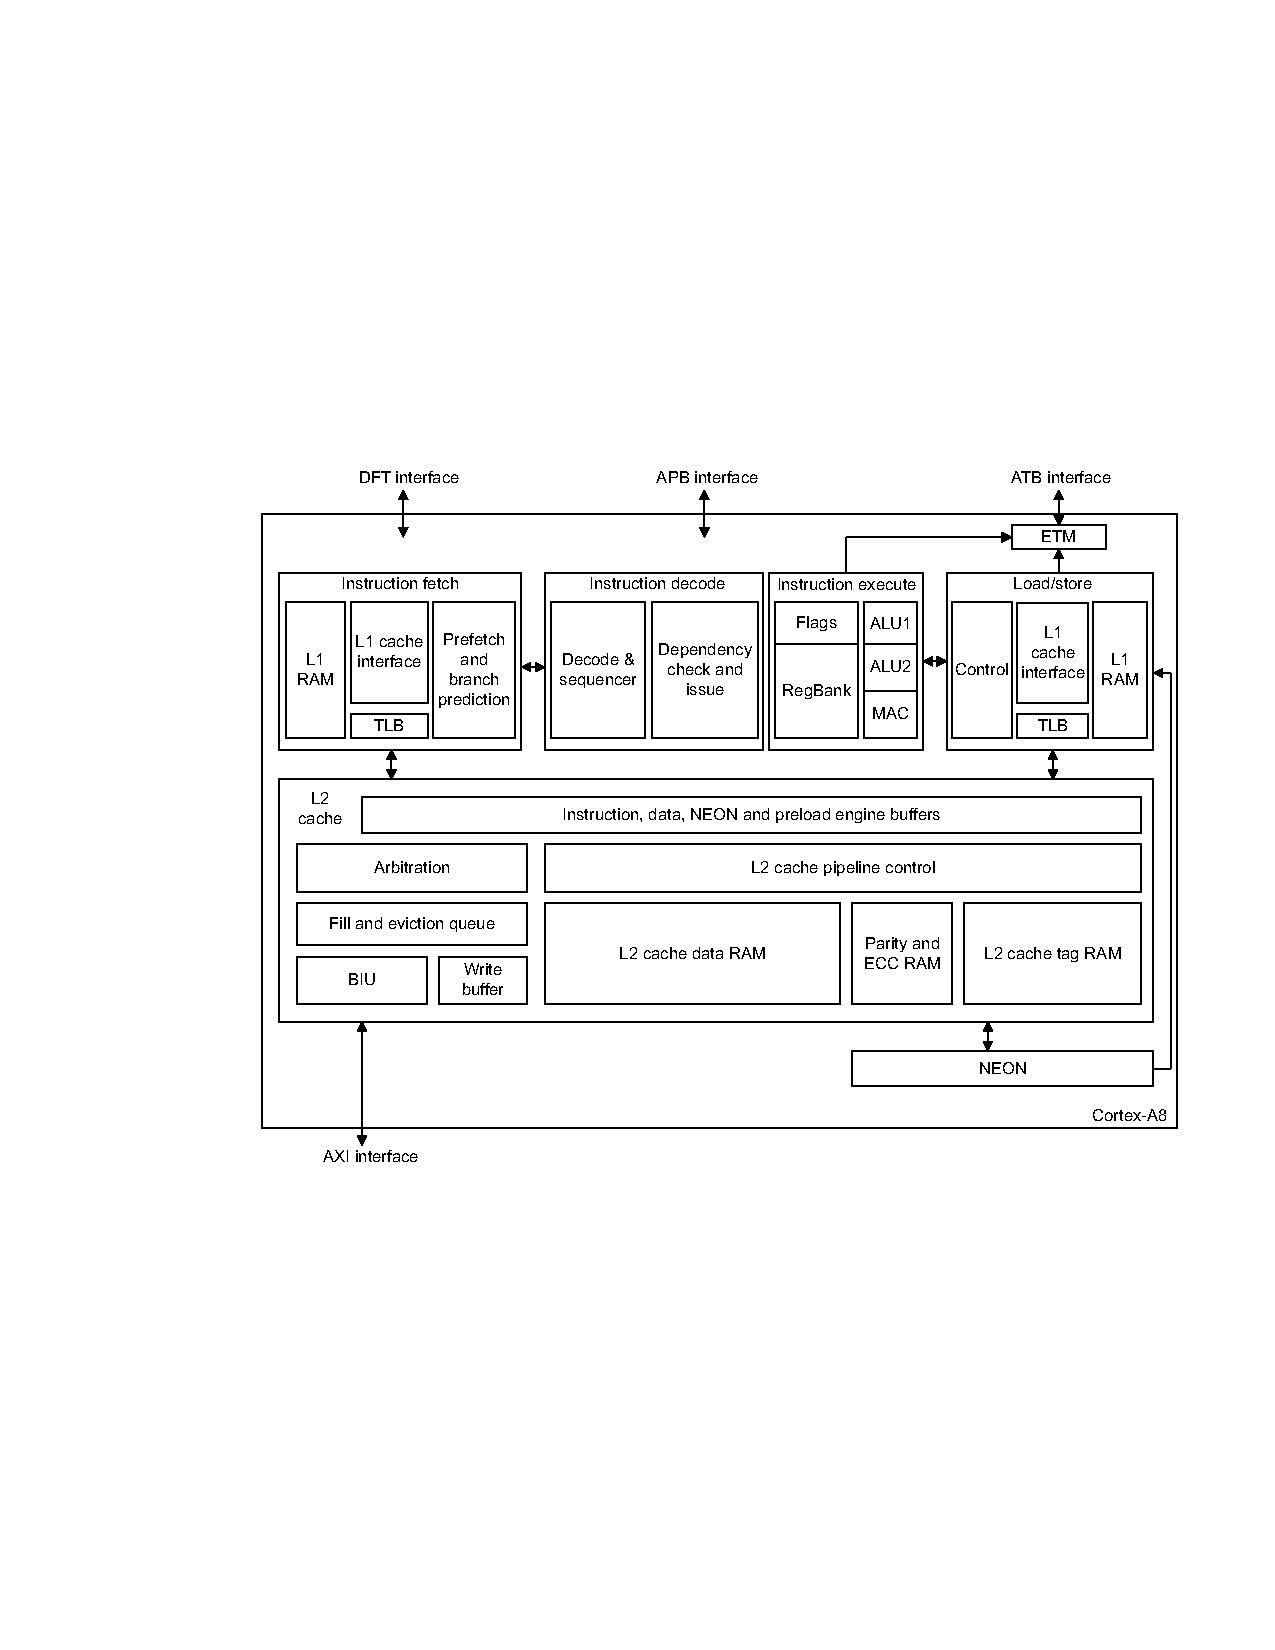
\includegraphics{./fig/CortexA8.pdf}
	\caption{Overview of the Cortex-A8 architecture from \cite[p. 1-4]{A8Ref}.}
	\label{fig:cortexa8}
\end{figure}

\section{Main Features}
A1

\section{Registers}
A2

Register Format
Word Length
Access Methods

Virtual memory and cache?


\begin{table}[htbp]
	\centering
	\begin{tabular}{lllllll}
		\toprule
		Type						&	\multicolumn{3}{l}{Name}	&	Preserved	&	Notes						\\
		\midrule
	 	General-purpose register	&	\multicolumn{3}{l}{R0}		&	No			&	Argument/result/scratch 1   \\
							 		&	\multicolumn{3}{l}{R1}		&	No			&	Argument/result/scratch 2   \\
							 		&	\multicolumn{3}{l}{R2}		&	No			&	Argument/scratch 3			\\
							 		&	\multicolumn{3}{l}{R3}		&	No			&	Argument/scratch 4			\\
							 		&	\multicolumn{3}{l}{R4}		&	Yes			&	Variable register 1			\\
							 		&	\multicolumn{3}{l}{R5}		&	Yes			&	Variable register 2			\\
							 		&	\multicolumn{3}{l}{R6}		&	Yes			&	Variable register 3			\\
							 		&	\multicolumn{3}{l}{R7}		&	Yes			&	Variable register 4 / Frame pointer on iOS	\\
							 		&	\multicolumn{3}{l}{R8}		&	Yes			&	Variable register 5			\\
							 		&	\multicolumn{3}{l}{R9}		&	Special		&	Platform register			\\
							 		&	\multicolumn{3}{l}{R10}		&	Yes			&	Variable register 7			\\
							 		&	\multicolumn{3}{l}{R11}		&	Yes			&	Variable register 8			\\
							 		&	\multicolumn{3}{l}{R12}		&	No			&	The Intra-Procedure-call scratch register (IP)	\\
							 		&	\multicolumn{3}{l}{R13}		&	Special		&	Stack pointer (SP)	 		\\
							 		&	\multicolumn{3}{l}{R14}		&	Special		&	Link register (LR)	 		\\
							 		&	\multicolumn{3}{l}{R15}		&	Special		&	Program counter (PC) 		\\
		Program status register		&	\multicolumn{3}{l}{CPSR}	&	Special		&						 		\\
		VFP / Advanced SIMD register&	Q0	&	D0	&	S0			&	No			&	  		\\
									&		&		&	S1			&	No			&	  		\\
									&		&	D1	&	S2			&	No			&	  		\\
									&		&		&	S3			&	No			&	  		\\
									&	Q1	&	D2	&	S4			&	No			&	  		\\
									&		&		&	S5			&	No			&	  		\\
									&		&	D3	&	S6			&	No			&	  		\\
									&		&		&	S7			&	No			&	  		\\
									&	Q2	&	D4	&	S8			&	No			&	  		\\
									&		&		&	S9			&	No			&	  		\\
									&		&	D5	&	S10			&	No			&	  		\\
									&		&		&	S11			&	No			&	  		\\
									&	Q3	&	D6	&	S12			&	No			&	  		\\
									&		&		&	S13			&	No			&	  		\\
									&		&	D7	&	S14			&	No			&	  		\\
									&		&		&	S15			&	No			&	  		\\
									&	Q4	&	D8	&	S16			&	Yes			&	  		\\
									&		&		&	S17			&	Yes			&	  		\\
									&		&	D9	&	S18			&	Yes			&	  		\\
									&		&		&	S19			&	Yes			&	  		\\
									&	Q5	&	D10	&	S20			&	Yes			&	  		\\
									&		&		&	S21			&	Yes			&	  		\\
									&		&	D11	&	S22			&	Yes			&	  		\\
									&		&		&	S23			&	Yes			&	  		\\
									&	Q6	&	D12	&	S24			&	Yes			&	  		\\
									&		&		&	S25			&	Yes			&	  		\\
									&		&	D13	&	S26			&	Yes			&	  		\\
									&		&		&	S27			&	Yes			&	  		\\
									&	Q7	&	D14	&	S28			&	Yes			&	  		\\
									&		&		&	S29			&	Yes			&	  		\\
									&		&	D15	&	S30			&	Yes			&	  		\\
									&		&		&	S31			&	Yes			&	  		\\
		VFP status register			&	\multicolumn{3}{l}{FPSCR}	&	Special		&						 		\\
		\bottomrule
	\end{tabular}
	\caption{User-mode registers. Compiled from \cite[p. 15]{AAPCS} and \cite[p. 14--15]{iOSABI}.}
	\label{tab:registers}
\end{table}


\begin{figure}[h]
	\centering
	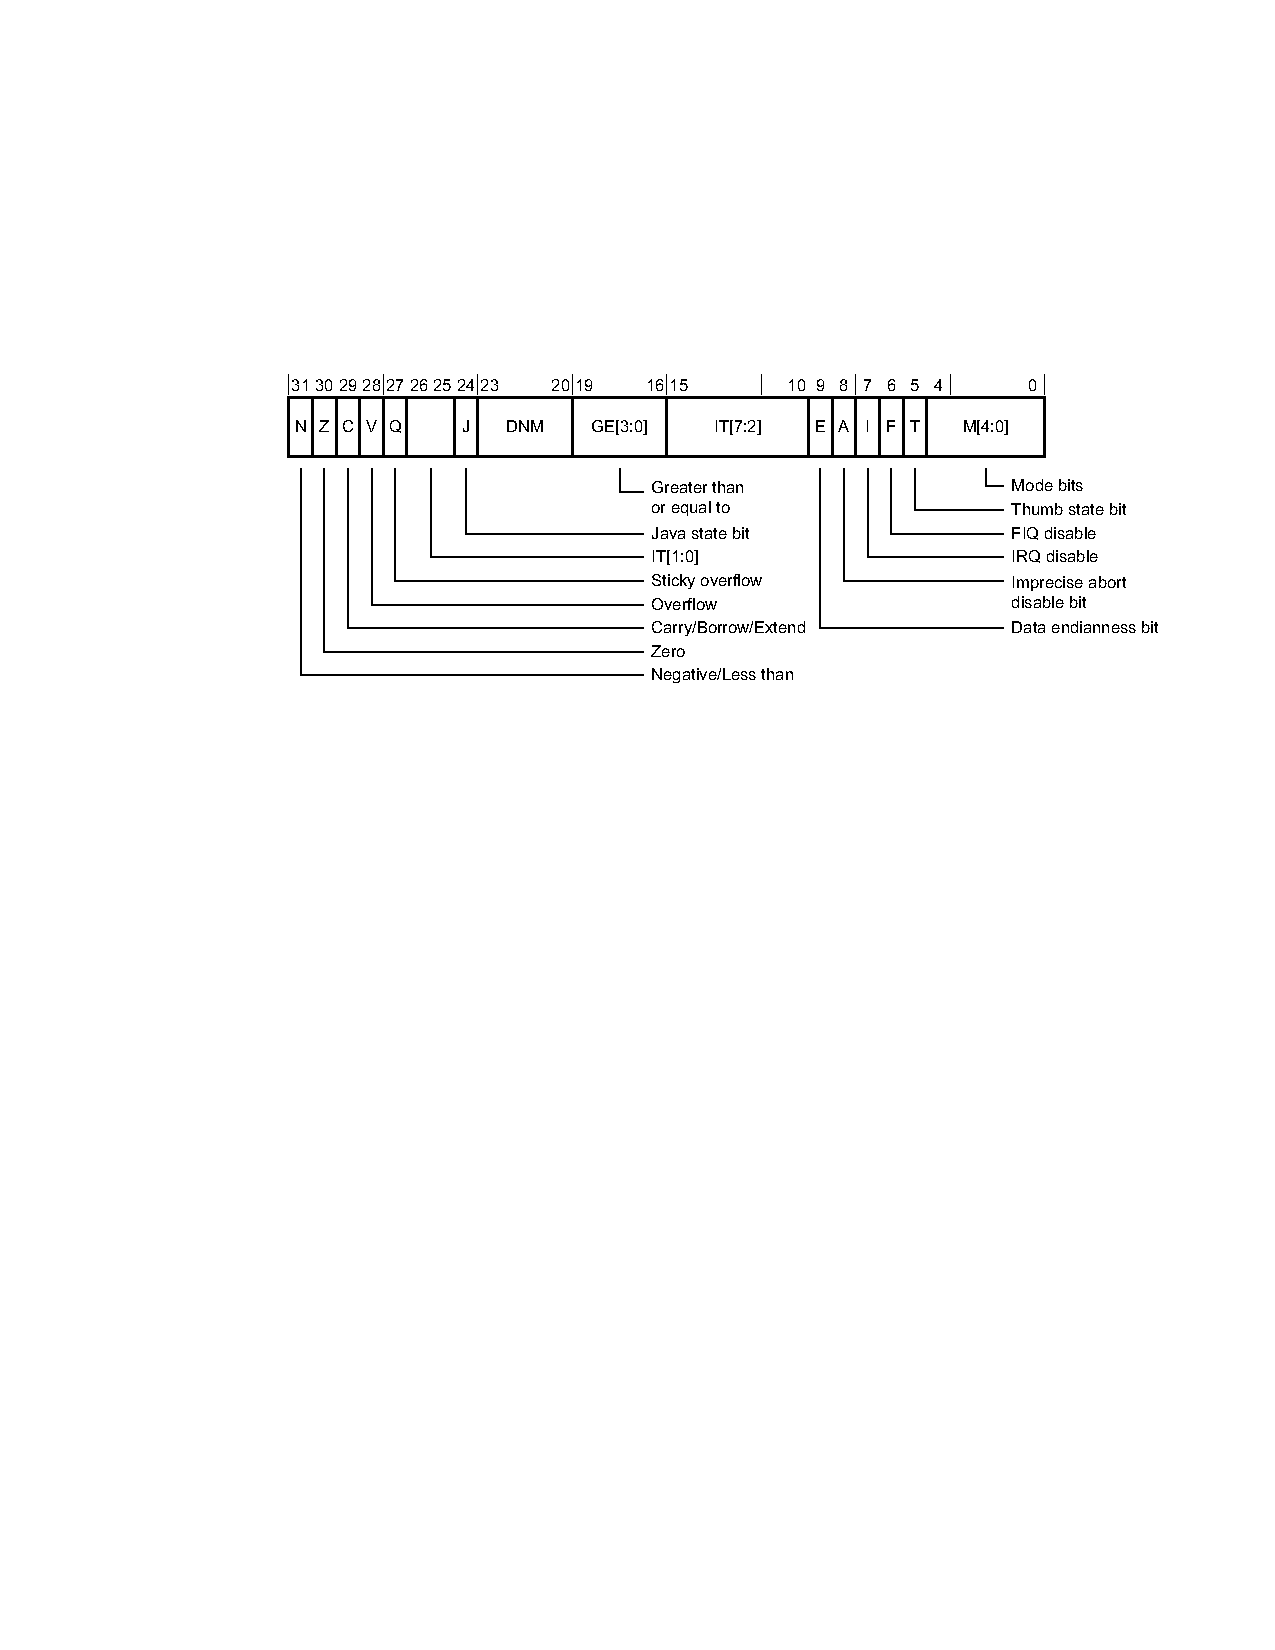
\includegraphics{./fig/CPSR.pdf}
	\caption{Program status register from \cite[p. 2-21]{A8Ref}.}
	\label{fig:cpsr}
\end{figure}


\section{Data Types}

\begin{table}[htbp]
	\centering
	\begin{tabular}{lr}
		\toprule
		Type			&		Size		\\
		\midrule
		doubleword		&		64-bit		\\
		word			& 		32-bit		\\
		halfword 		& 		16-bit		\\
		byte 			& 		8-bit		\\
		\bottomrule
	\end{tabular}
	\caption{Table caption}
	\label{tab:typesizes}
\end{table}

unsigned is two's complement

mixed-endian (E-bit in Program Status Register) and unaligned support but should be aligned for best performance
2.14


A2
A3
2-14
\section{Instruction Format}
instruction order
ARM
Thumb
ThumbEE

conditional instructions
APSR

A4
A5.1
Condition execution A8-8
\section{Unusual Instructions}
Perhaps in A4.4.6, A4.4.7, A4.8
bit fields?
\section{Memory Management}
A3
B2

6-2
\section{ARM Assembly Programming Example}
iOS ABI Function Call Guide\cite{iOSABI}

\renewcommand*{\refname}{\section{References}}
\bibliographystyle{plain}
\bibliography{ARM_Report}

\clearpage

\appendix
\section{ARM Assembly Programming Example -- Inner Product of Two Vectors}
  
\lstinputlisting[language={[ARM]Assembler}]{../ARM/dot_product.s}

\end{document}
